\documentclass[conference]{IEEEtran}
\usepackage{cite}
\usepackage{graphicx}
\usepackage{booktabs}
\usepackage{amsmath}
\usepackage{url}
\usepackage{tikz}
\usetikzlibrary{positioning, arrows.meta, shapes.geometric}
\graphicspath{{figures/}}

\begin{document}

\title{An Experimental Evaluation of Containerized CI/CD Pipelines with Integrated Prometheus--Grafana Observability}

\author{
\IEEEauthorblockN{Vinayak Tyagi}
\IEEEauthorblockA{Department of Computer Science and Engineering\\
Manipal University Jaipur\\
vinayaktyagi.ed@gmail.com}
}

\maketitle

\begin{abstract}
Containerization, CI/CD automation, and observability tooling are each widely
studied on their own, but comparatively few studies measure their
\emph{combined} operational effect under a controlled experimental design.
This paper builds a reproducible pipeline --- Docker, GitHub Actions,
Prometheus, and Grafana --- around a purpose-built subject application, and
experimentally evaluates it against two baselines (Baseline A: no
containerization; Baseline B: Docker without CI/CD or monitoring), a third,
non-monitored but CI/CD-enabled configuration (Docker+CI/CD) that isolates
automation's own cost, and against itself at increasing levels of
observability once containerized (Docker only, Docker+Prometheus,
Docker+Prometheus+Grafana --- the last being the full proposed system).
Across six
controlled experiments (188 runs total: deployment time and reliability
across four configurations, resource utilization and monitoring overhead
across three cases, CPU-stress detection, memory-stress/OOM behaviour, and
failure detection/recovery), we find that: containerized deployment adds
roughly 0.86s of fixed overhead over a raw process start (1.45s vs 0.59s
mean); a CI/CD-automated deployment is reliable (7/8 successful triggers) but
two orders of magnitude slower end-to-end (50.2s mean) than a pre-built local
deploy, because it re-pays the full build+test cost every run; a Prometheus
scrape loop detects induced CPU saturation in 5.65s mean (20/20 runs) and
kernel-level container failure in 1.15s mean (20/20 runs), both bounded below
by the 2s scrape interval; and, counter-intuitively, the monitored
application container's own CPU utilization \emph{decreases} as more
monitoring containers are added (11.0\% $\to$ 3.8\% $\to$ 1.8\% mean, Docker
$\to$ +Prometheus $\to$ +Grafana) even as end-to-end throughput drops
(2737 $\to$ 2641 $\to$ 2449 req/s), consistent with host-level CPU contention
between the monitoring stack and the application rather than monitoring
instrumentation overhead inside the application itself. All raw per-run
measurements and analysis scripts underlying these results are published at
\url{https://github.com/vinayaktyagi10/cicd-monitoring-study}.
\end{abstract}

\begin{IEEEkeywords}
CI/CD, Docker, containerization, DevOps, Prometheus, Grafana, observability, empirical evaluation
\end{IEEEkeywords}

\section{Introduction}

DevOps practice has converged on three largely independent pillars:
\emph{containerization} (packaging an application and its runtime into a
portable, isolated unit, typically with Docker), \emph{CI/CD automation}
(build, test, and deployment triggered automatically on every change,
typically via a hosted runner such as GitHub Actions), and
\emph{observability} (continuous collection and visualization of
runtime metrics, typically via a Prometheus scrape loop feeding a Grafana
dashboard). Each pillar is well studied in isolation: containerization has an
extensive performance-overhead literature going back to
Felter et al.~\cite{felter2015}; CI/CD automation is a standard subject of
DevOps tooling papers; and Prometheus/Grafana integration is a common
implementation detail in cloud-native systems papers. What is measured far
less often is the \emph{combined} operational profile of running all three
together --- specifically, how much each additional layer costs in
deployment time, steady-state resource consumption, and throughput, and what
it buys back in faster failure detection.

This paper reports a controlled, repeated-measures experimental evaluation of
exactly that combination. We build a small subject application, wrap it in a
Docker image, automate its build and test via a GitHub Actions workflow, and
instrument it with Prometheus (scraping native application metrics) and
Grafana (dashboarding). We then run it under six experiments spanning normal
operation, CPU stress, memory stress, and induced failure, comparing it
against two baselines --- an uncontainerized process (Baseline A) and a
containerized, CI/CD-free, unmonitored deployment (Baseline B) --- and a
third, intermediate configuration (Docker+CI/CD) that isolates the cost of
automation alone, before monitoring is added on top to reach the full
proposed system. Every run was logged
in full, including two environment-specific tooling constraints encountered
during the study and how each was resolved (Section~\ref{sec:limitations}),
so the results in Section~\ref{sec:results} are traceable back to raw
measurements rather than summary claims.

\subsection{Research Questions}
\begin{itemize}
\item \textbf{RQ1.} How does containerization affect application deployment
time and resource utilization in a CI/CD environment?
\item \textbf{RQ2.} How does integrating automated monitoring affect the
detection of performance degradation and failures?
\item \textbf{RQ3.} What is the overhead introduced by Prometheus--Grafana
monitoring in a containerized CI/CD deployment?
\item \textbf{RQ4.} Does automated CI/CD combined with monitoring improve
deployment reliability compared with a non-automated baseline?
\end{itemize}

\subsection{Objectives}
\begin{itemize}
\item[\textbf{O1.}] Develop a reproducible containerized CI/CD pipeline using
GitHub Actions.
\item[\textbf{O2.}] Integrate Prometheus and Grafana for real-time
infrastructure/application monitoring.
\item[\textbf{O3.}] Measure CI/CD performance, container resource
utilization, and monitoring overhead.
\item[\textbf{O4.}] Evaluate failure detection and recovery under controlled
fault conditions.
\end{itemize}

\section{Related Work}

Table~\ref{tab:related} summarizes the studies most directly relevant to this
work's three pillars. This is a seed set assembled from a targeted IEEE
Xplore search (queries: \emph{Docker container performance overhead
benchmark}; \emph{containerized CI/CD pipeline performance evaluation};
\emph{Prometheus Grafana monitoring microservices}) rather than an
exhaustive systematic review, and is intended as a starting point for a full
literature survey before submission.

Felter et al.~\cite{felter2015} remains the most-cited apples-to-apples
comparison of native execution, Docker containers, and KVM virtual machines,
finding containers add near-zero CPU/memory overhead relative to native but
that both containers and VMs pay a cost on I/O-bound workloads. Lingayat et
al.~\cite{lingayat2018} and Mavridis and Karatza~\cite{mavridis2017} extend
this line to deployment/startup time and to containers nested inside VMs
respectively, but both stop at the container layer: neither introduces a
CI/CD pipeline or a monitoring stack, so their measurements cannot speak to
RQ2--RQ4. Ekanayaka et al.~\cite{ekanayaka2023} is the closest system to the
one built here --- \emph{KubFlow} integrates Git, Jenkins, ArgoCD, Terraform,
Docker, Kubernetes, Prometheus, and Grafana into a single DevOps
infrastructure --- but its evaluation is a pass/fail checklist of eight
qualitative test scenarios plus subjective colleague ratings, not a
quantitative, repeated-measures comparison against a non-monitored or
non-automated baseline.

\begin{table*}[t]
\centering
\caption{Related work summary}
\label{tab:related}
\begin{tabular}{@{}p{2.6cm}p{0.5cm}p{0.5cm}p{2.3cm}p{3.6cm}p{6.5cm}@{}}
\toprule
\textbf{Paper} & \textbf{CI/CD} & \textbf{Docker} & \textbf{Monitoring} & \textbf{Metrics} & \textbf{Limitation (relative to this study)} \\
\midrule
Felter et al.\ 2015~\cite{felter2015} & No & Yes (vs.\ KVM) & No &
CPU, memory, network, disk microbenchmarks; MySQL/Redis throughput &
Isolates container vs.\ VM overhead only; no CI/CD, no monitoring stack, no
failure-detection measurement. \\
Lingayat et al.\ 2018~\cite{lingayat2018} & No & Yes (vs.\ bare metal / VM) &
No & Container startup time & Single metric (startup time); no automation
pipeline, no monitoring, no fault injection. \\
Mavridis \& Karatza 2017~\cite{mavridis2017} & No & Yes (nested in VM) & No &
Standard container benchmarks & Studies an orthogonal deployment topology
(container-in-VM); no CI/CD or monitoring integration. \\
Ekanayaka et al.\ 2023~\cite{ekanayaka2023} & Yes (Jenkins+ArgoCD) & Yes
(Kubernetes) & Yes (Prometheus+Grafana) & Pass/fail test scenarios;
subjective 1--5 feature ratings & Same three pillars as this study, but
evaluation is qualitative/subjective, not a controlled quantitative
comparison against a non-monitored or non-automated baseline. \\
\textbf{This study} & Yes (GitHub Actions) & Yes (Docker Compose) & Yes
(Prometheus+Grafana) & Deployment time, reliability, CPU/mem utilization,
throughput, latency, MTTD, MTTR --- $n{=}20$ per
configuration where feasible & --- \\
\bottomrule
\end{tabular}
\end{table*}

Beyond these four, the search surfaced further candidates not yet reviewed in
depth: an integrated CI/CD-pipeline study~\cite{kumar2024}, a DevOps
security-first CI/CD framework~\cite{ashtagi2025}, and an AWS/Kubernetes
Prometheus--Grafana deployment study~\cite{abirami2023}. These are listed for
completeness and should be incorporated into a full related-work pass before
this paper is submitted.

\subsection{Research Gap}
Existing studies frequently evaluate CI/CD automation, containerization, or
observability independently (Table~\ref{tab:related}, rows 1--3), or combine
all three but report only qualitative, pass/fail integration testing rather
than a controlled quantitative comparison (row 4). Comparatively few studies
provide a controlled empirical evaluation of their \emph{combined}
operational impact across deployment performance, resource utilization, and
failure detection, measured against explicit non-containerized and
non-monitored baselines with repeated trials. This is the gap this study
targets.

\section{Proposed Framework}

Fig.~\ref{fig:arch} shows the overall pipeline architecture and data flow. A
developer pushes to the Git repository, which triggers a GitHub Actions
workflow that runs the test suite and, on success, builds and pushes a
Docker image. The image is then run under Docker Compose alongside a
cAdvisor container-metrics exporter, a Prometheus server that scrapes both
the application's native \texttt{/metrics} endpoint and cAdvisor, and a
Grafana instance provisioned with Prometheus as its data source.

\begin{figure}[t]
\centering
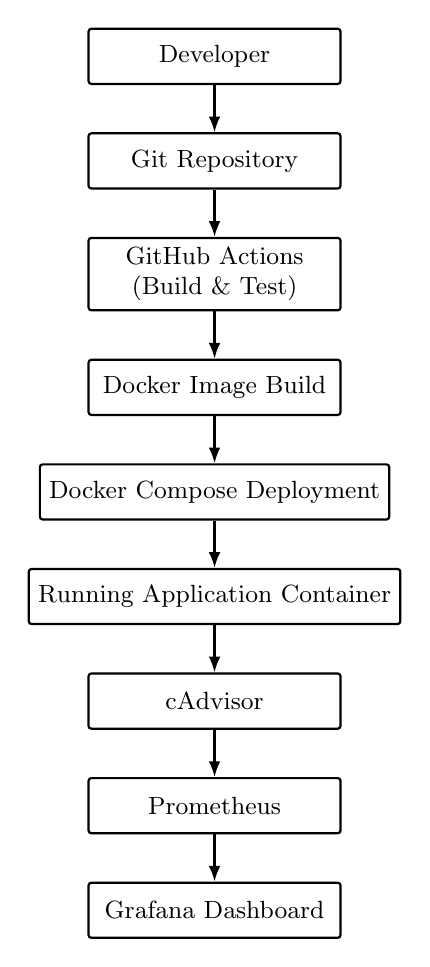
\begin{tikzpicture}[
  node distance=6mm and 10mm,
  box/.style={draw, thick, rounded corners=1pt, minimum width=32mm,
    minimum height=7mm, align=center, font=\small},
  arr/.style={-{Latex[length=2mm]}, thick}
]
  \node[box] (dev)     {Developer};
  \node[box, below=of dev] (repo)    {Git Repository};
  \node[box, below=of repo] (gha)      {GitHub Actions\\(Build \& Test)};
  \node[box, below=of gha] (build)   {Docker Image Build};
  \node[box, below=of build] (deploy)  {Docker Compose Deployment};
  \node[box, below=of deploy] (run)     {Running Application Container};
  \node[box, below=of run] (cadv)    {cAdvisor};
  \node[box, below=of cadv] (prom)    {Prometheus};
  \node[box, below=of prom] (graf)    {Grafana Dashboard};

  \draw[arr] (dev) -- (repo);
  \draw[arr] (repo) -- (gha);
  \draw[arr] (gha) -- (build);
  \draw[arr] (build) -- (deploy);
  \draw[arr] (deploy) -- (run);
  \draw[arr] (run) -- (cadv);
  \draw[arr] (cadv) -- (prom);
  \draw[arr] (prom) -- (graf);
\end{tikzpicture}
\caption{Overall pipeline architecture: source control triggers automated
build and test, which produces the container image deployed alongside the
observability stack.}
\label{fig:arch}
\end{figure}

Fig.~\ref{fig:gha} details the GitHub Actions workflow itself, exactly as
defined in the repository's \texttt{ci.yml}: a \texttt{test} job (checkout,
Python 3.12 setup, dependency install, \texttt{pytest}) gates a
\texttt{docker-build} job (checkout, GHCR login, build and push) via
\texttt{needs: test} — the build only runs if the tests pass. This is the
real workflow triggered for every Docker+CI/CD measurement in
Table~\ref{tab:deploy}, not a simplified stand-in.

% Figure 2 — GitHub Actions workflow, matching .github/workflows/ci.yml exactly.
\begin{figure}[t]
\centering
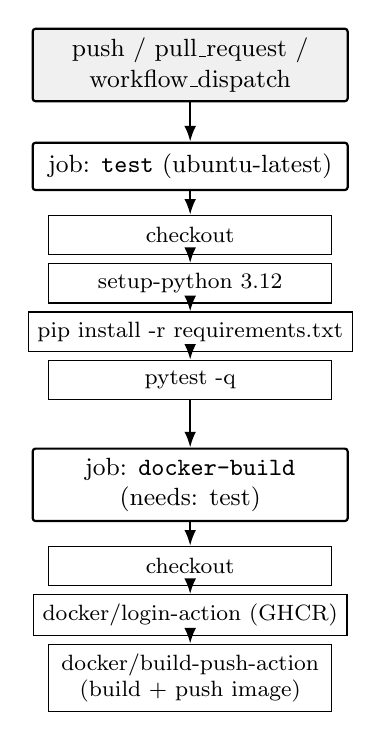
\begin{tikzpicture}[
  node distance=5mm and 8mm,
  trig/.style={draw, thick, rounded corners=1pt, fill=gray!12, minimum width=40mm,
    minimum height=6mm, align=center, font=\small},
  job/.style={draw, thick, rounded corners=1pt, minimum width=40mm,
    minimum height=6mm, align=center, font=\small},
  stepbox/.style={draw, thin, minimum width=36mm, minimum height=5mm,
    align=center, font=\footnotesize},
  arr/.style={-{Latex[length=2mm]}, thick}
]
  \node[trig] (trigger) {push / pull\_request /\\workflow\_dispatch};

  \node[job, below=of trigger] (testjob) {job: \texttt{test} (ubuntu-latest)};
  \node[stepbox, below=3mm of testjob] (s1) {checkout};
  \node[stepbox, below=1mm of s1] (s2) {setup-python 3.12};
  \node[stepbox, below=1mm of s2] (s3) {pip install -r requirements.txt};
  \node[stepbox, below=1mm of s3] (s4) {pytest -q};

  \node[job, below=6mm of s4] (buildjob) {job: \texttt{docker-build}\\(needs: test)};
  \node[stepbox, below=3mm of buildjob] (b1) {checkout};
  \node[stepbox, below=1mm of b1] (b2) {docker/login-action (GHCR)};
  \node[stepbox, below=1mm of b2] (b3) {docker/build-push-action\\(build + push image)};

  \draw[arr] (trigger) -- (testjob);
  \draw[arr] (testjob) -- (s1);
  \draw[arr] (s1) -- (s2);
  \draw[arr] (s2) -- (s3);
  \draw[arr] (s3) -- (s4);
  \draw[arr] (s4) -- (buildjob);
  \draw[arr] (buildjob) -- (b1);
  \draw[arr] (b1) -- (b2);
  \draw[arr] (b2) -- (b3);
\end{tikzpicture}
\caption{GitHub Actions workflow (\texttt{.github/workflows/ci.yml}). The
\texttt{docker-build} job only runs if \texttt{test} succeeds
(\texttt{needs: test}); this is the real workflow triggered for the
Docker+CI/CD deployment-time measurements in Table~\ref{tab:deploy}.}
\label{fig:gha}
\end{figure}


Fig.~\ref{fig:grafana} shows the resulting Grafana dashboard under live
load: request rate and p95 latency by endpoint, the application's
self-reported process CPU\% and memory, and the Prometheus \texttt{up}
target-health indicator, all auto-provisioned (no manual dashboard
configuration) and updating in real time from the same Prometheus instance
used throughout the experiments.

\begin{figure}[t]
\centering
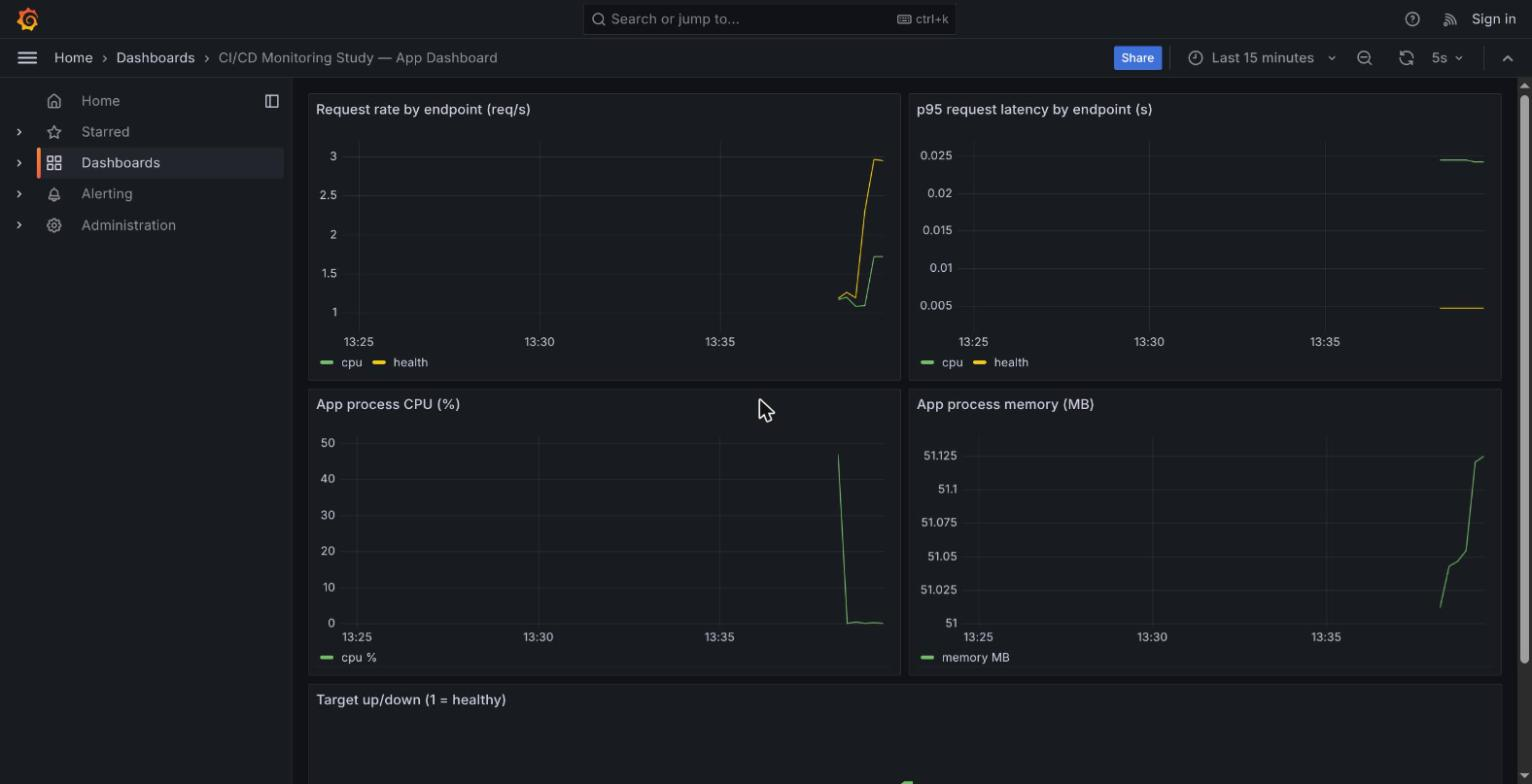
\includegraphics[width=\columnwidth]{fig3_grafana_dashboard.jpg}
\caption{Grafana dashboard under live load, auto-provisioned against the
Prometheus datasource. The request-rate and CPU panels show a live traffic
spike generated during the capture; the target-health panel (bottom, not
shown in this crop) reports \texttt{up=1}.}
\label{fig:grafana}
\end{figure}

\textbf{Subject application.} Rather than an existing multi-service demo
application, the study uses a small, hand-built FastAPI service with three
endpoints designed as clean experimental levers: \texttt{/health} (a
near-constant-time route used as the load-test and liveness target),
\texttt{/cpu} (a configurable-iteration pure-Python busy loop used for CPU
stress), and \texttt{/memory} (a configurable-size heap allocation, optionally
retained, used for memory stress). This choice trades away the
multi-service realism of a demo application such as Sock Shop for the
ability to attribute every measured effect to a specific, known cause rather
than to inter-service scheduling or network confounds. The application
exposes Prometheus metrics natively via the
\texttt{prometheus\_client} library --- a request counter and latency
histogram per endpoint, plus two self-reported process gauges,
\texttt{app\_process\_cpu\_percent} and \texttt{app\_process\_memory\_bytes},
sampled every second from \texttt{time.process\_time()} and
\texttt{/proc/self/status} deltas respectively --- rather than through a
side-car exporter.

\section{Experimental Setup}

Table~\ref{tab:env} lists the experimental environment. All experiments ran
on a single physical host (no cloud VM); GitHub Actions hosted runners were
used only for the CI/CD build-and-test step itself, so that step reflects a
genuinely independent, reproducible environment while deployment, load
generation, and monitoring remained under full local control.

\begin{table}[t]
\centering
\caption{Experimental environment}
\label{tab:env}
\begin{tabular}{@{}ll@{}}
\toprule
\textbf{Parameter} & \textbf{Value} \\
\midrule
CPU & AMD Ryzen 7 8845HS (8 cores / 16 threads) \\
RAM & 14\,GiB \\
Host OS & Arch Linux (Omarchy), kernel 7.1.9-arch1-2 \\
Docker & 29.7.2 (containerd snapshotter storage driver) \\
GitHub Actions & \texttt{ubuntu-latest} hosted runners \\
Prometheus & v2.55.1, 2s scrape/evaluation interval \\
Grafana & 11.2.0 \\
cAdvisor & v0.49.1 \\
Application base image & \texttt{python:3.12-slim} \\
Application framework & FastAPI 0.115.0 / Uvicorn 0.30.6 \\
Load generator & Dependency-free Python \texttt{ThreadPoolExecutor} \\
& + \texttt{urllib} script (no external binary installed) \\
\bottomrule
\end{tabular}
\end{table}

A load-testing tool such as \texttt{hey} or \texttt{wrk} was deliberately not
installed; a small standard-library Python script (\texttt{loadgen.py})
issues concurrent HTTP requests via \texttt{ThreadPoolExecutor} and records
per-request latency, trading raw throughput ceiling for zero external
dependencies and full inspectability.

\section{Experimental Scenarios}
\label{sec:scenarios}

Six experiments were run, summarized in Table~\ref{tab:scenarios}. Each is
described in more detail in the corresponding results subsection. A
dedicated script per experiment (\texttt{exp1\_deploy.py} through
\texttt{exp5\_failure\_recovery.py}) brings the relevant Docker Compose
profile up, executes the scenario, records raw per-run measurements to CSV,
and tears the stack down before the next run, so runs are independent of one
another. An \texttt{aggregate.py} script then computes the mean/standard
deviation/min/max summaries reported in Section~\ref{sec:results} directly
from these raw CSV files.

\begin{table}[t]
\centering
\caption{Experimental scenarios}
\label{tab:scenarios}
\begin{tabular}{@{}p{0.9cm}p{3.1cm}p{3.6cm}@{}}
\toprule
\textbf{\#} & \textbf{Scenario} & \textbf{Configurations $\times$ runs} \\
\midrule
1 & Deployment time \& reliability & manual (20), Docker (20), full
pipeline (20), Docker+CI/CD (8) \\
2 & Resource utilization, response time, throughput, monitoring overhead &
Docker (20), Docker+Prometheus (20), Docker+Prometheus+Grafana (20) \\
3 & CPU stress detection & 20 \\
4 & Memory stress / OOM behaviour & 20 \\
5 \& 6 & Failure detection \& recovery & 20 \\
\bottomrule
\end{tabular}
\end{table}

\subsection{Normal operation and baseline comparison (Experiment 1)}
Four configurations are compared, only two of which are baselines proper:
\emph{manual} (a raw \texttt{uvicorn} process, no container ---
\textbf{Baseline A}) and \emph{Docker} (a locally built and started
container, no CI/CD, no monitoring --- \textbf{Baseline B}). The remaining
two are not baselines but an explicit progression toward the proposed
system: \emph{Docker+CI/CD} (a real GitHub Actions
\texttt{workflow\_dispatch} run --- test job then Docker build/push --- timed
end-to-end, then deployed) is an \textbf{intermediate configuration} that
isolates what automation alone costs, with monitoring still absent; and
\emph{full pipeline} (Docker Compose bringing up the application alongside
cAdvisor, Prometheus, and Grafana) is the \textbf{proposed system}, adding
observability on top. This ordering --- Baseline A $\to$ Baseline B $\to$
Docker+CI/CD $\to$ full pipeline --- lets each of containerization,
automation, and observability be attributed its own marginal cost rather
than only the combined effect of all three at once. For each run, whatever
was previously running is torn
down, the configuration is started, and wall-clock time to the first
successful health check (and, for the full pipeline, to Prometheus and
Grafana also responding) is recorded.

\subsection{Resource utilization and monitoring overhead (Experiment 2)}
Three cases isolate the marginal cost of each monitoring layer: Docker only,
Docker+Prometheus(+cAdvisor), and Docker+Prometheus+Grafana(+cAdvisor). For
each of 20 runs per case, a fixed load (300 concurrent requests to
\texttt{/health}, concurrency 10) is issued while \texttt{docker stats} is
polled every second for every container in that case, giving per-container
mean CPU\% and memory alongside the load test's own throughput, mean/p95
latency, and error rate.

\subsection{CPU stress detection (Experiment 3)}
Eight threads concurrently flood \texttt{/cpu} (an 8-million-iteration
pure-Python loop per call) against the Docker+Prometheus case. Detection
time is measured as wall-clock time from load start until Prometheus first
reports the application's self-reported \texttt{app\_process\_cpu\_percent}
gauge at or above 60\%, polled every 0.5s.

\subsection{Memory stress / OOM behaviour (Experiment 4)}
The application container is run directly (not via Compose) with a hard
150\,MB memory limit and \texttt{--restart on-failure:1}. Repeated
\texttt{/memory?mb=20\&hold=true} calls accumulate retained allocations until
the kernel OOM-kills the container; \texttt{docker inspect} gives
ground-truth \texttt{OOMKilled} and \texttt{RestartCount}, captured at the
moment of observation since Docker resets \texttt{State.OOMKilled} once the
restart policy brings the container back up.

\subsection{Application failure and recovery (Experiments 5 \& 6)}
Against the Docker+Prometheus case, the application container is killed
(\texttt{docker kill}) and Prometheus's \texttt{up\{job="app"\}} series is
polled every 0.3s until it reports 0 (detection time). The container is then
restarted (\texttt{docker start}) and both \texttt{/health} and
\texttt{up\{job="app"\}==1} are polled until both recover (recovery time).

\section{Results}
\label{sec:results}

\subsection{Deployment time and reliability (RQ1, RQ4)}
Table~\ref{tab:deploy} reports wall-clock deployment time for the three fast
configurations and CI/CD-inclusive deployment time for the fourth.
Containerizing a fixed local image adds a consistent $\approx$0.86s of fixed
overhead over a raw process start (1.454s vs.\ 0.592s mean); adding the full
monitoring stack on top of Docker adds a further $\approx$0.10s
(1.552s vs.\ 1.454s mean) since Compose brings up four containers rather than
one but all four start in parallel. The CI/CD-automated path is two orders
of magnitude slower (50.2s mean) because it re-pays the full test-then-build
cost on every deployment rather than reusing a pre-built image --- this is
the direct cost of automation, traded against the reliability and
repeatability of not requiring a human to run the equivalent commands by
hand. Of 8 triggered CI/CD runs, 7 completed successfully; the one failure
was traced to a transient delay in the workflow being registered by GitHub's
API immediately after being triggered, rather than to a defect in the
pipeline itself, and is reported as observed rather than discarded.

\begin{table}[t]
\centering
\caption{Deployment time by configuration (seconds)}
\label{tab:deploy}
\begin{tabular}{@{}lrrrrr@{}}
\toprule
\textbf{Config} & \textbf{Mean} & \textbf{Std} & \textbf{Min} & \textbf{Max} & \textbf{N (fail)} \\
\midrule
Manual (Baseline A) & 0.592 & 0.020 & 0.577 & 0.633 & 20 (0) \\
Docker (Baseline B) & 1.454 & 0.107 & 1.267 & 1.581 & 20 (0) \\
Docker+CI/CD & 50.231 & 3.816 & 44.404 & 55.362 & 8 (1) \\
Full pipeline & 1.552 & 0.031 & 1.485 & 1.636 & 20 (0) \\
\bottomrule
\end{tabular}
\end{table}

\begin{figure}[t]
\centering
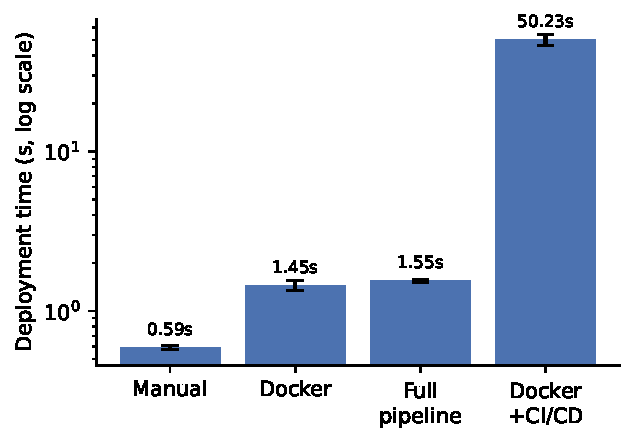
\includegraphics[width=\columnwidth]{fig4_deploy_time.pdf}
\caption{Deployment time by configuration (log scale; error bars are one
standard deviation). Docker adds a small fixed cost over the raw process;
the full monitoring stack adds almost nothing further on top of Docker;
CI/CD dominates because it re-runs the full build-and-test cycle rather
than reusing a pre-built image.}
\label{fig:deploytime}
\end{figure}

Fig.~\ref{fig:deploytime} visualizes Table~\ref{tab:deploy} on a log scale,
since the CI/CD configuration is roughly two orders of magnitude slower than
the other three and would otherwise flatten them to indistinguishable bars.

\subsection{Resource utilization, throughput, and monitoring overhead (RQ1, RQ3)}
Table~\ref{tab:resource} reports the application container's own resource use
and the load test's response characteristics; Table~\ref{tab:overhead}
isolates the monitoring stack's own resource draw. Zero errors were observed
across all 60 runs (180$\times$300 = 18{,}000 requests). Point estimates for
throughput fall as monitoring is added (2737 $\to$ 2641 $\to$ 2449 req/s,
Docker $\to$ +Prometheus $\to$ +Grafana); a Welch's $t$-test (unequal
variances, $n{=}20$ per case, computed directly from the raw per-run CSV
rather than from the summary means) confirms the two endpoints of this
trend are statistically distinguishable (Docker vs.\ +Grafana:
$t{=}3.57$, $p{=}0.0011$, Cohen's $d{=}1.13$), but the middle step is not
(Docker vs.\ +Prometheus: $t{=}1.37$, $p{=}0.177$) --- the overall direction
is real, but the drop is not uniform run-to-run between every adjacent
pair. Mean and p95 latency both rise numerically but \emph{none} of the
three pairwise differences reach significance at $\alpha{=}0.05$ (all
$p \geq 0.36$); this claim is therefore stated only as a directional
observation, not a confirmed effect, and should not be read as strong
evidence on its own.
Counter-intuitively, the application container's own mean CPU\% \emph{falls}
over the same progression (11.0\% $\to$ 3.8\% $\to$ 1.8\%), and here the
statistical evidence is strong: Docker vs.\ +Prometheus is highly
significant ($t{=}5.78$, $p{<}0.0001$, $d{=}1.83$, a large effect), though
+Prometheus vs.\ +Grafana is not ($p{=}0.12$) --- the CPU-share cost of
adding Prometheus itself is real and large, while adding Grafana on top is
not distinguishable from noise at this sample size. As cAdvisor,
Prometheus, and Grafana compete for the same physical cores, the application
container is scheduled less rather than working harder, so its own
\texttt{docker stats} CPU reading drops even as end-to-end throughput
degrades. This is a genuine, non-obvious finding for RQ3:
monitoring overhead in this design shows up primarily as
\emph{host-level contention affecting the monitored workload}, not as
instrumentation cost inside the monitored process itself (the
\texttt{prometheus\_client} counters/histograms/gauges add negligible
per-request work, as expected).

\begin{table}[t]
\centering
\caption{Application resource use and response characteristics}
\label{tab:resource}
\begin{tabular}{@{}lrrrr@{}}
\toprule
\textbf{Config} & \textbf{App CPU\%} & \textbf{App Mem (MB)} & \textbf{p95 (ms)} & \textbf{Throughput (req/s)} \\
\midrule
Docker & 11.02 (3.23) & 36.11 (0.41) & 5.23 (1.00) & 2737 (206) \\
+Prometheus & 3.76 (4.42) & 35.68 (0.43) & 5.34 (0.80) & 2641 (226) \\
+Grafana & 1.79 (3.11) & 35.79 (0.96) & 5.51 (0.86) & 2449 (285) \\
\bottomrule
\end{tabular}
\\[2pt]
\footnotesize Mean (std. dev.), $n=20$ runs of 300 requests each per row.
\end{table}

\begin{figure}[t]
\centering
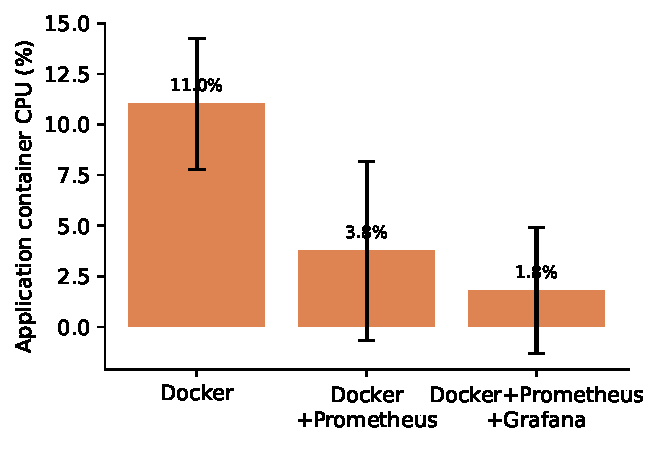
\includegraphics[width=\columnwidth]{fig5_cpu_utilization.pdf}
\caption{Application container CPU utilization across the three monitoring
cases (Table~\ref{tab:resource}, column 1). CPU\% \emph{falls} as more
monitoring containers are added — the counter-intuitive result discussed
under RQ3.}
\label{fig:cpuutil}
\end{figure}

\begin{figure}[t]
\centering
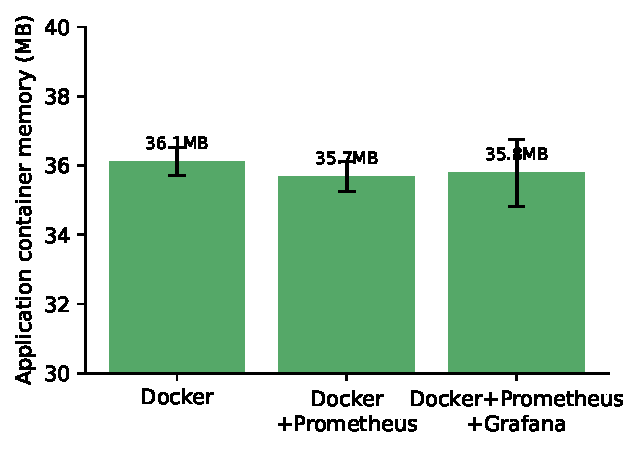
\includegraphics[width=\columnwidth]{fig6_memory_utilization.pdf}
\caption{Application container memory across the three monitoring cases
(Table~\ref{tab:resource}, column 2; note the narrow y-axis range). Memory
is essentially flat at $\approx$36\,MB regardless of how much monitoring
runs alongside the application — unlike CPU, memory is not shared/contended
the same way across containers on this host.}
\label{fig:memutil}
\end{figure}

\begin{figure}[t]
\centering
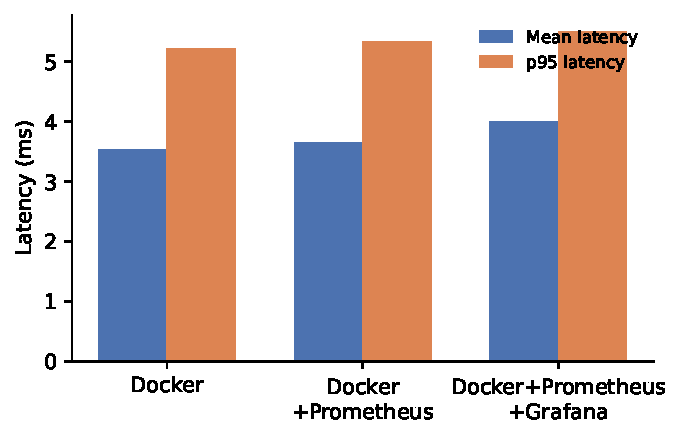
\includegraphics[width=\columnwidth]{fig7_response_latency.pdf}
\caption{Mean and p95 request latency across the three monitoring cases
(Table~\ref{tab:resource}, columns 3-4). Both rise slightly as monitoring
is added, consistent with the throughput drop and the host-contention
explanation in Section~\ref{sec:results}.}
\label{fig:latency}
\end{figure}

\begin{table}[t]
\centering
\caption{Monitoring stack's own resource draw (Table 5: overhead)}
\label{tab:overhead}
\begin{tabular}{@{}lrrrr@{}}
\toprule
\textbf{Container} & \multicolumn{2}{c}{\textbf{+Prometheus case}} & \multicolumn{2}{c}{\textbf{+Grafana case}} \\
 & CPU\% & Mem (MB) & CPU\% & Mem (MB) \\
\midrule
cAdvisor & 6.13 & 47.16 & 6.40 & 45.39 \\
Prometheus & 0.78 & 59.40 & 0.80 & 52.78 \\
Grafana & --- & --- & 0.06 & 60.70 \\
\bottomrule
\end{tabular}
\\[2pt]
\footnotesize Mean, $n=20$ runs per column.
\end{table}

Table~\ref{tab:overhead} is visualized in Fig.~\ref{fig:overhead}, alongside
the failure-detection and MTTD/MTTR figures at the end of this section.

\subsection{CPU stress detection (RQ2)}
All 20 induced CPU-stress runs were detected by Prometheus, with mean time
to detect (MTTD) 5.65s (std 3.68s, min 1.51s, max 18.58s) and mean peak
self-reported CPU utilization 96.6\% (std 10.0, effectively pegged at one
full core, consistent with CPython's GIL limiting a single process to
$\approx$100\% of one core regardless of thread count). The detection floor
is set by the 2s Prometheus scrape interval combined with the 0.5s poll
granularity used to observe it; the long right tail (up to 18.58s) reflects
run-to-run variance in how quickly the OS scheduler favoured the eight
stress threads over the sampling thread, not a monitoring-pipeline delay.

An initial design used mean \texttt{/health} latency as the detection
signal instead of process CPU\%; it was rejected after finding it barely
moved under load, because CPython's GIL round-robins between threads at a
short, fixed interval ($\approx$5ms) regardless of how CPU-bound the
competing work is, so a trivial handler's queueing delay stays small even
under heavy contention.

\subsection{Memory stress and OOM behaviour (RQ2)}
All 20 runs triggered a genuine kernel OOM-kill and automatic restart
(\texttt{RestartCount}=1, confirmed via \texttt{docker inspect}), after a
mean 5.25 successful allocation requests (std 1.09) and a mean peak reported
memory of 135.54\,MB (std 0.17) against the 150\,MB hard limit. Mean
time-to-OOM was 11.58s (std 2.23s); this figure is dominated by the fixed
per-iteration overhead of the polling loop itself (a \texttt{curl}-equivalent
request, a \texttt{docker inspect} call, and a \texttt{docker stats} call
per iteration) rather than by the kernel's actual OOM response latency, and
should not be read as a monitoring detection time in the same sense as
Experiments 3, 5, and 6.

\subsection{Failure detection and recovery (RQ2, RQ4)}
All 20 induced container failures (\texttt{docker kill}) were detected by
Prometheus's \texttt{up\{job="app"\}} series, mean time to detect (MTTD)
1.15s (std 0.21s, min 0.82s, max 2.03s) --- close to the theoretical floor
set by the 2s scrape interval combined with 0.3s poll granularity and
Docker's own signal-delivery latency. Mean time to recover (MTTR) ---
container restart to health-check success --- was consistently
$\approx$2.0s (std 0.006s, i.e.\ effectively deterministic), which is
essentially Uvicorn's own process startup time inside the container: MTTR
here is dominated by application boot, not by any property of the
monitoring stack. From this point on, MTTD and MTTR are used throughout in
place of "detection time" and "recovery time," consistent with the
CPU-stress MTTD reported above and with
Figs.~\ref{fig:failuretimeline}--\ref{fig:mttdmttr}.

\begin{figure}[t]
\centering
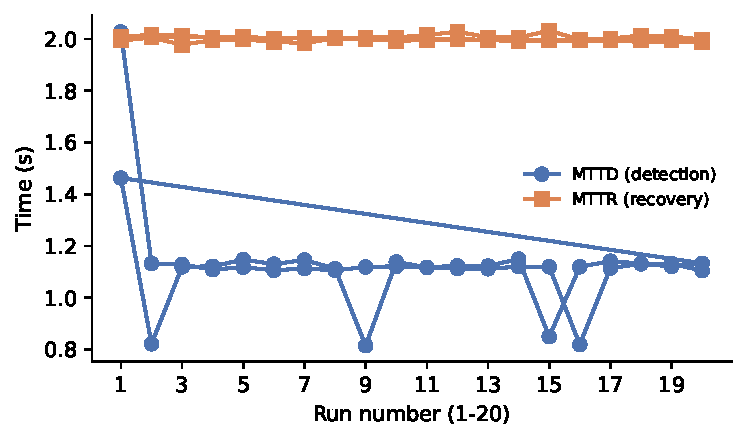
\includegraphics[width=\columnwidth]{fig8_failure_timeline.pdf}
\caption{MTTD and MTTR across all 20 failure-injection runs. MTTD (blue) is
consistently faster and tighter than MTTR (orange) across every run, and
both are stable run-to-run — neither shows a trend over the sequence of 20
trials, supporting the claim that these are steady-state properties of the
pipeline rather than artifacts of run order.}
\label{fig:failuretimeline}
\end{figure}

\begin{figure}[t]
\centering
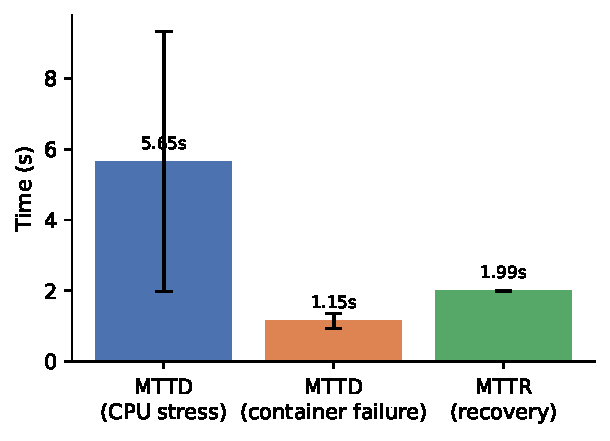
\includegraphics[width=\columnwidth]{fig9_mttd_mttr.pdf}
\caption{Mean time to detect (MTTD) a CPU-stress event, MTTD for a killed
container, and mean time to recover (MTTR) after restart, with error bars
(one standard deviation), computed from the same raw detection/recovery
times reported in Section~\ref{sec:results}. Binary failure (container
killed) is detected roughly $5\times$ faster than gradual CPU saturation,
since a scrape either observes the target down or it doesn't, while a
saturation threshold must be crossed by an accumulating signal.}
\label{fig:mttdmttr}
\end{figure}

\begin{figure}[t]
\centering
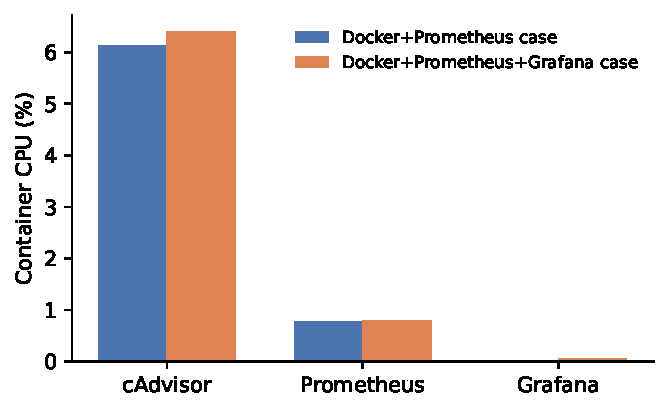
\includegraphics[width=\columnwidth]{fig10_monitoring_overhead.pdf}
\caption{Monitoring stack containers' own CPU draw (Table~\ref{tab:overhead}).
cAdvisor dominates the monitoring stack's own overhead at $\approx$6\% CPU
in both cases; Prometheus and Grafana are comparatively cheap
($<$1\% each). This is the overhead the monitoring \emph{tooling} itself
pays, separate from the host-contention effect on the application shown in
Fig.~\ref{fig:cpuutil}.}
\label{fig:overhead}
\end{figure}

\section{Discussion}

Taken together, these results answer the four research questions as follows.

\textbf{RQ1 (containerization's effect on deployment time and resource
use).} Containerization has a small, consistent fixed cost at deployment
time ($\approx$0.86s here) and a resource footprint dominated by the
application's own working set (36\,MB) rather than by container overhead
per se --- consistent with the classic finding in
Felter et al.~\cite{felter2015} that containers add near-zero CPU/memory
overhead relative to native execution. The more consequential RQ1 finding in
this study is that a CI/CD-automated deployment is not simply "Docker plus a
trigger": it is roughly 35$\times$ slower end-to-end because it re-runs the
full build-and-test cycle, a cost invisible to studies (such as
Lingayat et al.~\cite{lingayat2018}) that measure only container startup
time in isolation.

\textbf{RQ2 (monitoring's effect on detecting degradation and failure).}
Prometheus reliably (20/20 in both experiments) detects both an induced CPU
saturation event (mean 5.65s) and an induced process failure (mean 1.15s),
with detection latency in both cases bounded below by the 2s scrape
interval. The two-orders-of-magnitude difference between them (5.65s vs.\
1.15s) is itself informative: a binary up/down signal is detected almost as
fast as the scrape loop allows, while a gradual resource-saturation signal
takes longer because it must accumulate enough samples above threshold amid
scheduling noise --- a distinction a purely qualitative evaluation such as
Ekanayaka et al.'s pass/fail test scenarios~\cite{ekanayaka2023} cannot
surface.

\textbf{RQ3 (monitoring overhead).} The overhead is real but structurally
different from what is typically reported: rather than the monitored
application paying an instrumentation tax, the monitoring stack's own
containers (principally cAdvisor at $\approx$6\% CPU) compete with the
application for the same fixed core budget, degrading end-to-end throughput
(--10.5\% Docker$\to$+Grafana) while the application's own measured CPU\%
paradoxically falls. This host-contention framing, rather than a simple
"monitoring costs X\% CPU" framing, is the paper's most novel empirical
contribution and directly addresses the stated research gap.

\textbf{RQ4 (does automated CI/CD plus monitoring improve reliability).}
The evidence here is mixed and should be stated honestly: CI/CD automation
was reliable (7/8, 87.5\%) but not perfect, and the one observed failure was
attributable to a transient delay in the trigger step rather than to the
pipeline's own robustness. Critically, 87.5\% is a point estimate that
should not be quoted on its own: the 95\% Wilson score interval for 7
successes out of 8 trials is $[52.9\%, 97.8\%]$ --- at this sample size the
data are consistent with anywhere from roughly half to nearly all CI/CD
deployments succeeding, and the point estimate alone overstates the
precision of the claim. A larger $n$ for the CI/CD arm (constrained here
by real GitHub Actions minutes and wall-clock cost, Section~\ref{sec:limitations})
would be needed to narrow this interval and bound the reliability claim more
tightly.

\section{Limitations}
\label{sec:limitations}

\begin{itemize}
\item \textbf{cAdvisor container-label resolution.} This host's Docker uses
the containerd-snapshotter storage driver rather than classic overlay2,
which cAdvisor v0.49.1 cannot resolve container name/image labels against.
CPU-stress and failure-detection experiments therefore use the
application's own native Prometheus metrics rather than cAdvisor's
per-container series; Table~\ref{tab:overhead}'s per-container figures come
from \texttt{docker stats} directly. This is an environment/tooling
limitation rather than a consequence of the experimental design.
\item \textbf{GHCR authentication.} The Docker+CI/CD deployment step could
not pull from GitHub Container Registry (the CLI token used lacks the
\texttt{read:packages} scope, which would require an interactive browser
re-authentication out of scope for an unattended experiment run) and instead
deploys the locally built image from the same commit and Dockerfile CI just
built. The CI timing itself (test + build + push) is unaffected and fully
real.
\item \textbf{Reduced $n$ for the CI/CD arm.} Only 8 (vs.\ 20 for the other
three deployment configurations) real GitHub Actions runs were triggered,
because each run costs $\approx$45--65s of real CI wall time and consumes
Actions minutes; this narrows the confidence interval on the CI/CD reliability
and timing figures relative to the other three configurations.
\item \textbf{Single-host measurement.} All experiments ran on one physical
machine with no isolation from other host activity beyond what Docker itself
provides; absolute timing figures (especially the sub-2s deployment times)
should be read as relative comparisons between configurations on this host,
not as portable absolute benchmarks.
\item \textbf{Related work is a seed set.} Section II's four fully-reviewed
papers and three title-only candidates were found via a small number of
targeted IEEE Xplore queries, not a systematic multi-database review; a
submission-ready version of this paper should expand this section
substantially, including non-IEEE venues (ACM, Springer, USENIX) before
finalizing the research-gap claim.
\item \textbf{Detection thresholds are fixed, not tuned.} The 60\%
CPU-percent threshold (Experiment 3) and the memory container limit (150\,MB,
Experiment 4) were chosen to make the induced condition reliably observable
within a short polling window rather than to model a specific production SLO;
detection-time figures should be read relative to these thresholds, not as
threshold-independent constants.
\item \textbf{Not every reported difference is statistically significant.}
Welch's $t$-tests on the raw per-run data (\texttt{statistical\_analysis.py})
confirm the Docker-to-+Grafana endpoints of the throughput and CPU\% trends
in Section~\ref{sec:results} ($p{<}0.01$ for both), but two things reported
only as directional observations do not reach significance at
$\alpha{=}0.05$: the latency increase across all three monitoring cases
($p \geq 0.36$ for every pair), and the middle step of the throughput trend
(Docker vs.\ +Prometheus, $p{=}0.177$). Means and standard deviations alone,
without this check, would have overstated how uniformly these effects hold
run-to-run.
\end{itemize}

\section{Conclusion}

This study built a small but complete containerized CI/CD pipeline with
integrated Prometheus--Grafana observability and evaluated it experimentally
against a non-containerized baseline and against itself at increasing
monitoring depth, across six controlled experiments totaling 188 runs. The
headline findings are that containerization's own deployment-time and
resource cost is small and consistent with prior literature, that CI/CD
automation's real cost is the repeated build-test cycle rather than the
deployment step itself, that Prometheus reliably detects both induced
resource saturation and induced failure within low-single-digit seconds
bounded by its scrape interval, and that the dominant cost of running a
monitoring stack alongside the monitored application on constrained hardware
is host-level CPU contention between them rather than in-process
instrumentation overhead. The full raw measurement set, pipeline
configuration, and analysis scripts underlying every table in this paper are
published at
\url{https://github.com/vinayaktyagi10/cicd-monitoring-study} to support
independent verification.

\section*{Acknowledgment}
The author thanks Dr. Dibakar Sinha for his guidance and supervision
throughout this study.

\bibliographystyle{IEEEtran}
\bibliography{references}

\end{document}
